\documentclass{beamer}

\mode<presentation>
{
	\usetheme{default}      
	\usecolortheme{default} 
	\usefonttheme{default}  
	\setbeamertemplate{navigation symbols}{}
	\setbeamertemplate{caption}[numbered]
} 

\usepackage[english,russian]{babel}
\usepackage[utf8]{inputenc}
\usepackage[T1]{fontenc}
\usepackage{lmodern}
\usepackage{tikz}
\usepackage{array}
\usepackage{adjustbox}
\usepackage{pgfplots}
\pgfplotsset{compat=1.18}
\usepackage[T2A]{fontenc}  % Изменили на T2A для правильной поддержки кириллицы
\usepackage{cmap}          % Для улучшенного поиска в PDF
\usepackage{mathtext}      % Для правильного отображения математических символов в кириллице

\title{\huge Методы верификации кэша второго уровня графического процессора общего назначения}
\author{\fontsize{10}{12}\selectfont Кулевич Анастасия Юрьевна \\ Научный руководитель: Козлов Вячеслав Константинович \\ Научный консультант: Маслов Максим Владимирович}
\institute{\vskip 1cm Московский Физико-Технический Институт }
\date{2026}

\begin{document}
	
	\begin{frame}
		\titlepage
	\end{frame}
	
	\begin{frame}{Функциональная верификация}
		
		\begin{block}{Вызовы}
			\begin{itemize}
				\item Количество состояний системы
				\item Отсутствие способа доказать полную корректность
				\item Ограниченные сроки
			\end{itemize}
		\end{block}
		
	\end{frame}
	
	\begin{frame}{Постановка задачи}
		
		Ведётся разработка первого отечественного GPGPU.
		
		L2 кэш \--- один из ключевых компонентов.
		\begin{block}{Цель работы:}
			\begin{itemize}
				\item Изучение различных методов верификации
				\item Реализация методов для L2 кэша
				\item Сравнение методов 
			\end{itemize}
		\end{block}
		
	\end{frame}
	
	\begin{frame}{Методы, основанные на симуляции}
		
		\begin{block}{Походы:}
			\begin{itemize}
				\item Направленное тестирование
				\item Ограниченное случайное тестирование
				\item Трассы 
			\end{itemize}
		\end{block}
		
		\begin{figure}[htb]
			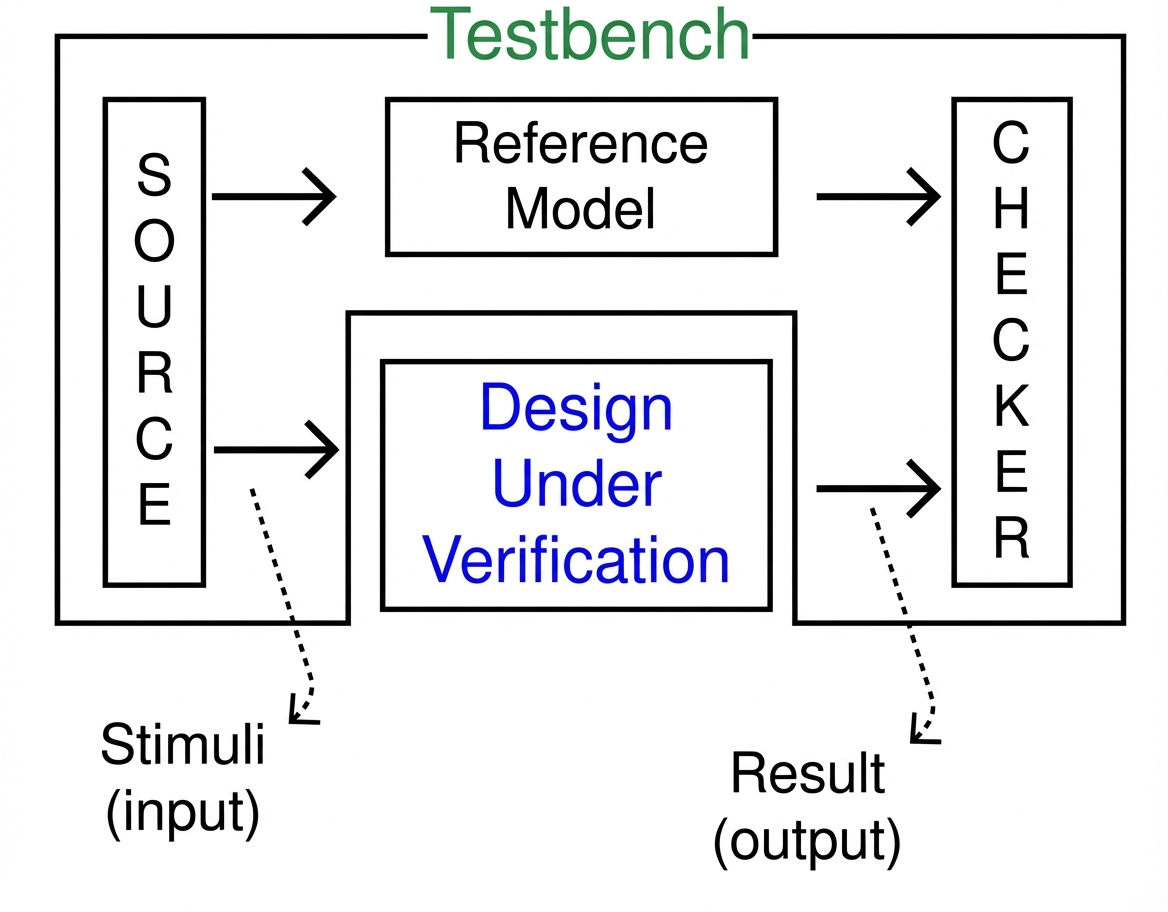
\includegraphics[width=.55\textwidth]{../src/img/testbench.png}
			\caption{\label{fig:tb}Общая структура тестбенча.}
		\end{figure}
		
	\end{frame}
	
	\begin{frame}{Ключевые особенности}
		
		\begin{itemize}
			\item Покрытие: 
				\begin{itemize}
					\item Функциональное
					\item Кодовое
				\end{itemize}
			\item Требуется много тестов
			\item Универсальность
		\end{itemize}
		
	\end{frame}
	
	\begin{frame}{Формальная верификация}
		
		\begin{block}{Алгоритм:}
			\begin{enumerate}
				\item[0.] Имеем формальное свойство $\phi$ и RTL-модуль $M$
				\item[1.] Создаем проверяющий автомат для $\neg \phi$.
				\item[2.] Извлекаем из $M$ конечный автомат $J$.
				\item[3.] Считаем произведение $J$ и $\phi$.
				\item[4.] Произведение содержит какой-либо путь (т.е. не пусто) => ошибка, найденный путь \--- контрпример.
				\item[5.] Если произведение пусто, то считаем, что $M$ удовлетворяет $\phi$.
			\end{enumerate}
		\end{block}
		
	\end{frame}
	
	\begin{frame}{Проблема комбинаторного взрыва}
		
		\begin{block}{Причины:}
			\begin{itemize}
				\item Последовательная логика
				\item Транспортировка данных 
				\item Трансформация данных
				\item Параметры
			\end{itemize}
		\end{block}
		
		\begin{block}{Решения:}
			\begin{itemize}
				\item Бинарная диаграмма решений
				\item Задача выполнимости булевых формул
				\item Редукция конуса влияния
			\end{itemize}
		\end{block}
		
	\end{frame}
	
	\begin{frame}{Ключевые особенности}
		
		\begin{block}{SystemVerilog Assertions (SVA):}
			\begin{itemize}
				\item assert()
				\item assume()
				\item cover()
			\end{itemize}
		\end{block}
		
		\begin{block}{Формальное покрытие:}
			\begin{itemize}
				\item Стимульное покрытие (stimuli coverage)
				\item Покрытие проверок (checker coverage)
			\end{itemize}
		\end{block}
		
	\end{frame}
	
	\begin{frame}{Устройство L2 кэша}
		
		\begin{figure}[htb]
			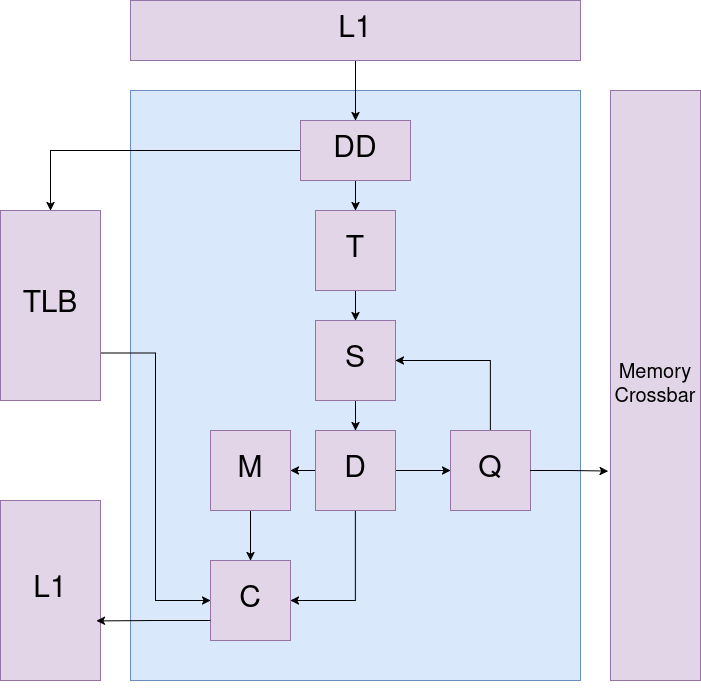
\includegraphics[width=.65\textwidth]{../src/img/l2.png}
			\caption{\label{fig:cache}Партиция L2 кэша GPGPU.}
		\end{figure}
		
	\end{frame}
	
	\begin{frame}{D-stage}
		
		\begin{columns}
			\begin{column}{0.5\textwidth}
				\begin{block}{Формальная верификация:}
					\begin{itemize}
						\item Проблема: массивный блок памяти
						\item Решение: замещение на модель
						\item Время: 4694 минут 
						
						($\approx 3$ суток)
					\end{itemize}
				\end{block}
				\vskip 3.9cm
				$ $
			\end{column}
			
			\begin{column}{0.5\textwidth}
				\begin{block}{Симуляция:}
					\begin{figure}[htb]
					\centering
					\begin{adjustbox}{max width=\textwidth}
						\begin{tikzpicture}
							\begin{axis}[
								xlabel={Количество транзакций},
								ylabel={Процент покрытия},
								xmin=0, xmax=48,
								ymin=0, ymax=110,
								xtick={0,3,9,15,21,27,33,39,45},
								ytick={0,20,40,60,80,100},
								legend pos=north west,
								ymajorgrids=true,
								grid style=dashed,
								]
								
								\addplot[smooth,
								tension=0.2,
								color=blue,
								mark=square,
								]
								coordinates {
									(0,0)
									(3,80.93)
									(6,88.48)
									(9,92.69)
									(12,94.1)
									(15,95.14)
									(18,95.66)
									(21,96.16)
									(24,96.63)
									(27,97.1)
									(30,97.53)
									(33,97.92)
									(36,98.24)
									(39,98.45)
									(42,98.58)
									(45,98.67)
								};
							\end{axis}
						\end{tikzpicture}
					\end{adjustbox}
					\caption{Процент кодового покрытия в зависимости от количества транзакций для D-stage}
					\label{fig:cov_d}
					\end{figure}
				\end{block}
			\end{column}
		\end{columns}
		
	\end{frame}
	
	\begin{frame}{T-stage}
		
		\begin{columns}
			\begin{column}{0.5\textwidth}
				\begin{block}{Формальная верификация:}
					\begin{itemize}
						\item Проблема: сложная последовательная логика
						\item Решение: разделение блока на части
						\item Время: 3752 минут 
						
						($\approx 2.5$ суток)
					\end{itemize}
				\end{block}
				\vskip 3.9cm
				$ $
			\end{column}
			
			\begin{column}{0.5\textwidth}
				\begin{block}{Симуляция:}
					\begin{figure}[htb]
						\centering
						\begin{adjustbox}{max width=\textwidth}
							\begin{tikzpicture}
								\begin{axis}[
									xlabel={Количество транзакций},
									ylabel={Процент покрытия},
									xmin=0, xmax=2200,
									ymin=0, ymax=110,
									xtick={0,400,800,1200,1600,2000},
									ytick={0,20,40,60,80,100},
									xticklabel style={
										/pgf/number format/1000 sep={}
									},
									legend pos=north west,
									ymajorgrids=true,
									grid style=dashed,
									]
									
									\addplot[smooth,
									tension=0.15,
									color=blue,
									mark=square,
									]
									coordinates {
										(0   ,0    )
										(200 ,94.53)
										(400 ,97.07)
										(600 ,98.22)
										(800 ,98.86)
										(1000,99.23)
										(1200,99.43)
										(1400,99.54)
										(1600,99.60)
										(1800,99.62)
										(2000,99.63)
									};
								\end{axis}
							\end{tikzpicture}
							\end{adjustbox}
							\caption{Процент кодового покрытия в зависимости от количества транзакций для T-stage}
							\label{fig:cov_t}
					\end{figure}
				\end{block}
			\end{column}
		\end{columns}
		
	\end{frame}
	
	\begin{frame}{Q-stage}
		
		\begin{columns}
			\begin{column}{0.5\textwidth}
				\begin{block}{Формальная верификация:}
					\begin{itemize}
						\item Проблема: много очередей (FIFO)
						\item Решение: разделение блока на части + дополнительная логика
						\item Время: 720 минут 
						
						(12 часов)
					\end{itemize}
				\end{block}
				\vskip 2.9cm
				$ $
			\end{column}
			
			\begin{column}{0.5\textwidth}
				\begin{block}{Симуляция:}
					\begin{figure}[htb]
						\centering
						\begin{adjustbox}{max width=\textwidth}
							\begin{tikzpicture}
								\begin{axis}[
									xlabel={Количество транзакций},
									ylabel={Процент покрытия},
									xmin=0, xmax=400,
									ymin=0, ymax=110,
									xtick={0,50,100,150,200,250,300,350},
									ytick={0,20,40,60,80,100},
									legend pos=north west,
									ymajorgrids=true,
									grid style=dashed,
									]
									
									\addplot[smooth,
									tension=0.2,
									color=blue,
									mark=square,
									]
									coordinates {
										(0  ,		0    )
										(10 ,		75.95)
										(20 ,		86.42)
										(30 ,		89.69)
										(40 ,		91.26)
										(50 ,		91.62)
										(60 ,		91.94)
										(70 ,		92.25)
										(80 ,		92.47)
										(90 ,		92.67)
										(100,		92.85)
										(110,		93.03)
										(120,		93.17)
										(130,		93.31)
										(140,		93.48)
										(150,		93.64)
										(160,		93.77)
										(170,		93.89)
										(180,		93.99)
										(190,		94.08)
										(200,		94.17)
										(210,		94.27)
										(220,		94.35)
										(230,		94.42)
										(240,		94.49)
										(250,		94.56)
										(260,		94.63)
										(270,		94.69)
										(280,		94.74)
										(290,		94.79)
										(300,		94.83)
										(310,		94.87)
										(320,		94.91)
										(330,		94.94)
										(340,		94.97)
										(350,		95   )
										(360,		95.02)
										(370,		95.04)
										(380,		95.05)
										(390,		95.06)
										
									};
								\end{axis}
							\end{tikzpicture}
							\end{adjustbox}
							\caption{Процент кодового покрытия в зависимости от количества транзакций для Q-stage.}
							\label{fig:cov_q}
					\end{figure}
				\end{block}
			\end{column}
		\end{columns}
		
	\end{frame}
	
	\begin{frame}{Сравнение методов}
		
		\begin{table}
		\small
			\begin{tabular}{l|r|r|r|r|r}
				Блок                                                              & D-stage            & C-stage & DD-stage & T-stage & Q-stage \\ \hline
				$N_{\text{триггеров}}$                                                        & 374 086             & 22 457   & 1788     & 79 936   & 35 906   \\ \hline
				$N_{\text{лог. вентилей}}$                                              & 1 074 060            & 142 640  & 34 599    & 271 233  & 195 514  \\ \hline
				$N_{\text{транзакций}}$ & 45 & 150 & 18 & 2000 & 390 \\ \hline 
				$t_{\text{сим}}$, с & 10                 & 12      & 10       & 201     & 19      \\ \hline
				$t_{\text{форм}}$, мин                         & 4694 & 1031    & 46       & 3752    & 720     \\ 
				
			\end{tabular}
			\caption{Время, затраченное на верификацию блоков используя методы формальной верификации и UVM-тестирования.}
			\label{tab:main-table}
		\end{table}
		
	\end{frame}
	
	\begin{frame}{Выводы}
		
		\begin{block}{Преимущества симуляции:}
			\begin{itemize}
				\item универсальность
				\item относительно низкий порог входа
				\item быстрота получения результатов для больших систем
			\end{itemize}
		\end{block}
		
		\begin{block}{Преимущества формальной верификации:}
			\begin{itemize}
				\item исчерпывающая проверка
				\item улучшенная локальность обнаружения ошибки
				\item быстрота получения результатов для малых систем
			\end{itemize}
		\end{block}
		
	\end{frame}
	
	\begin{frame}{Заключение}
		
		\begin{block}{Реализованы методы формальной верификации и симуляции для L2 кэша GPGPU:}
			\begin{itemize}
				\item симуляция \--- универсальный метод
				\item формальная верификация сталкивается с трудностями, но
				\item эффективнее в рамках применимости 
			\end{itemize}
		\end{block}
		
		\begin{block}{Дальнейшее развитие:}
			\begin{itemize}
				\item более углубленное изучение формальной верификации
				\item расширение исследования на другие компоненты
			\end{itemize}
		\end{block}
		
	\end{frame}
	
\end{document}